\documentclass{article}

\usepackage{graphicx}
\usepackage{parskip}
\usepackage{fullpage}
\usepackage{amsmath}
\usepackage{amsmath}
\usepackage{amsfonts}
\usepackage{amssymb}
\usepackage{enumitem}

\usepackage{listings}

\title{Quantum Mechanics Notes}
\author{Lucas Henry McConnell}

\begin{document}
\maketitle

\section{What is Quantum Mechanics}
\begin{quote}
``Deep in the human unconscious is a pervasive need for a logical universe that makes sense. But the real universe is always one step beyond logic.'' -- Frank Herbert
\end{quote}
\begin{figure}[h]
\centering{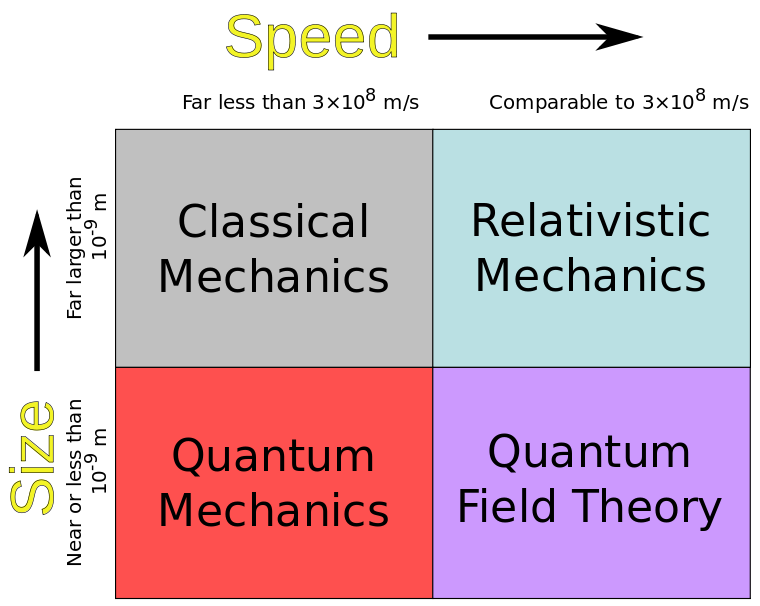
\includegraphics[scale=0.5]{cm_qm_gr_qft.png}}
\end{figure}
Quantum mechanics is a non-relativistic theory (meaning it breaks down as you approach the speed of light) and differs from classical mechanics on the basis that energy is a discrete rather than continuous quantity.
\newpage
\section{The beginnings of Quantum Mechanics}
\begin{quote}
For those who are not shocked when they first come across quantum theory cannot possibly have understood it. -- Niels Bohr
\end{quote}
Quantum mechanics is a little more intuitive if you get an idea of where it comes from. The first person to suggest that the energy levels of a physical system may be discrete was the Austrian physicist Ludwig Boltzmann, who suggested in 1877 that molecular energy levels may be discrete. Boltzmann was truly a visionary and pioneered a field of physics, now known as statistical mechanics\footnote{The better known field of thermodynamics is directly derived from statistical mechanics.}. Boltzmann's genius went largely unrecognised in his own lifetime. He was likely clinically depressed as a result of extremely low self-esteem and tragically committed suicide in 1906, at the age of 62. 

In 1900, some years after Boltzmann first hypothesised that energy could be discrete, German physicist Max Planck (very reluctantly) used tried using the idea of discrete energy to describe a famous unexplained phenomenon in physics known ``black body radiation''. To his great surprise, this actually worked and the idea that energy could be discrete spread rapidly through the physics community (most concentrated in Europe at that time). These discrete energy spacings can be regarded as little packets of energy and became known as quanta (singular quantum) and quantum mechanics was born. For this reason, Max Planck is regarded as the ``grandad'' of quantum mechanics.

Then in 1905, Max Planck's close friend, Albert Einstein (another German...), took inspiration from him and tried explaining the photoelectric effect by postulating that light (and actually all electromagnetic radiation) can be regarded as individual quanta of energy. These quanta of light came to be called photons. These are the basic light particles. At the time the photoelectric effect was deeply puzzling as it was widely believed that light was a type of wave\footnote{Numerous experiments demonstrated this. The most famous are Young's double slit experiments, where light clearly diffracts through slits as ripples in water might. Young was a bit of a polymath and actually helped translate the Rosetta stone.} and now Einstein was treating it as a particle. It is fairly well known today that light acts as both a wave and a particle, but at the time it was deeply disturbing as it violates the human need to neatly and distinctly categorise all phenomena.

Meanwhile in 1913, while all this was happening, other physicists will trying to deal with the problem of the atom. Classical mechanics predicts that point charges radiate power according to the Larmor formula:
\begin{equation}
P = \frac{2}{3} \frac{q^{2}a^{2}}{4\pi \epsilon_{0} c^{3}},
\end{equation}
where $a$ is its acceleration, $q$ is its charge, and $c$ is the speed of light. Now this formula is very problematic because if it's to be believed then matter shouldn't be stable. Take for example the hydrogen atom: in the classical picture, we have an electron orbiting a nucleus\footnote{It will experience acceleration towards the centre of its orbit from the centripedal force.} and as a point charge it radiates power according to the Larmor formula. But this means that, as it loses energy, it will spiral inwards and collapse into the nucleus, i.e. matter is unstable! But clearly most matter is stable so this can't be what's happening, or rather, it can't be the whole picture. The Danish physicist Niels Bohr tried his hand at fixing this. He used the idea of quantised energy to postulate the the atom must have discrete energy levels that correspond to particular orbits of the electron around the atom. So unlike a classical celestial mechanics problems where, given the right conditions of planet mass and distance, you can have any orbit, the hydrogen atom only permits a few discrete orbits and it can never collapse in on itself because it's energy cannot decrease beyond the lowest energy level and the hence the orbit it corresponds to. Bohr's model of the hydrogen atom forms part of what is called the \emph{old quantum mechanics}. This is not quantum mechanics as we will study it, but rather, some very clever people trying to beat classical mechanics into a quantum shape so that it works. Models such as these are said to be \emph{phenomenological}\footnote{According to \emph{wikipedia}: ``A phenomenological model is a scientific model that describes the empirical relationship of phenomena to each other, in a way which is consistent with fundamental theory, but is not directly derived from theory.'' Such models are still used very widely and when you don't have a nice theoretical model to describe something, they do the next best thing.}. This way of trying to ``force'' quantum effects onto a classical theory worked okay for the simple case of the hydrogen atom, but it failed to explain even the slightly more complex helium atom.

Then in 1923, French physicist Louis de Broglie, put forth his idea of \emph{matter waves}; the idea that particles can experience wave characteristics and vice versa. It was from this idea that modern quantum mechanics (or the new quantum mechanics) arose. German physicists  Werner Heisenberg, Max Born, and Pascual Jordan invented what is now called matrix quantum mechanics mechanics, while Austrian Erwin Schrodinger invented wave quantum mechanics. These are two equivalent ways of describing the same thing and Shrodinger showed as much in a famous paper. Both approaches are useful in their own way, not unlike the way calculus was developed independently by both Leibniz and Newton and each of their approaches has applications in which it seems most the natural.
\section{The Wave Function}
\begin{quote}
``I think I can safely say that nobody understands quantum mechanics.'' -- Richard Feynman
\end{quote}
The first and simplest formulation of classical mechanics was formulated by Newton. Newtonian mechanics is usually pretty intuitive. We all have a ``feel'' for what a force is and how forces should work. For a particle of mass $m$, the force acting on it is given by Newton's second law:
\begin{equation}
\mathbf{F} = m\mathbf{a},
\end{equation} 
where $\mathbf{F}$ is the force, $\mathbf{a}$ is the acceleration.

Quantum mechanics is a bit different. There are no forces. Instead, everything we want to know about a particle is provided by its \emph{wave function} $\Psi(x,t)$. We get the wave function by solving the Schrodinger equation:
\begin{equation}
\label{schrodinger_equation}
i \hbar \frac{\partial \Psi}{\partial t} = - \frac{\hbar^{2}}{2m}\frac{\partial^{2}\Psi}{\partial x^{2}} + V \Psi.
\end{equation}
Here $\hbar$ is Planck's constant\footnote{It's actually his original constant divided by 2$\pi$.} and $V$ is a scalar (as opposed to a vector) potential. Given suitable initial conditions $\Psi (x,0)$, then the Schrodinger equation determines $\Psi (x,t)$ for all future time. But where does the Schrodinger equation come from? Turns out he basically got it by clever guessing! He was trying to generalise de Broglie's idea of matter waves and ended up with this equation that accurately described quantum particles.

But what does the Schrodinger equation actually mean? Particle are localised in space, they are spread out like waves! The wave function should be understood in the context of the \emph{Born statistical interpretation}.  This says that the probability of finding the particle at point $x$, at time $t$ is given by $| \Psi(x,t) |^{2}$. The wave function is complex but remember that $|\Psi |^{2} = \Psi^{*}\Psi$, is real and non-negative (as a probability should be!). So technically:
\begin{equation}
\label{statistical_interpretation}
\int_{a}^{b} |\Psi(x,t)|^{2}dx = \left( \text{probability of finding the particle between $a$ and $b$, at time $t$.} \right)
\end{equation}
Probability is the area under the graph of $|\Psi|^{2}$ (see figure \ref{1}). Also, the wave function in figure \ref{1}, we will be far more likely to find the particle near $A$ (where $|\Psi|^{2}$ is large), than near $B$ (where $|\Psi|^{2}$ is small).
\begin{figure}[h]
\centering{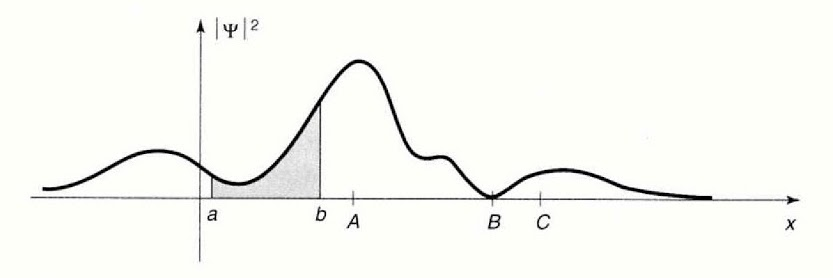
\includegraphics[scale=0.5]{griffiths_1.jpg}}
\caption{Illustration of a wave function.}
\label{1}
\end{figure}

The statistical interpretation is where quantum mechanics starts to go a bit weird on us. It gives us a kind of indeterminacy. Even if we know everything the theory has to tell us about a particle (i.e. its wave function), we cannot predict with any certainty the outcome of a simple experiment to measure, say, its position. All we have is statistical information. This is where the interpretation of quantum mechanics come in. It has been hotly debated among both physicists and philosophers as to whether the theory is defective or whether this is simply the way nature works. Let's say we set up an experiment to measure the position of the particle, and we find it at point $C$ (see figure \ref{1}). We may ask: where was the particle \emph{just} before we made the measurement? There have been historically three classifications of answers:
\begin{itemize}
\item The \emph{realist} postion: It was clearly at $C$, you fool!
\item The \emph{orthodox} position: The particle wasn't really anywhere. But measuring the particle, we have forced it assume a position.
\item The \emph{agnostic} postion: dunno
\end{itemize}

But what if we make a second measurement, \emph{immediately} after the first? On this question, all positions are in agreement. A repeated measurement on the same particle returns the same value. I mean, we can't really say the particle was at $C$ if, when we check again, its not there anymore. How does the orthodox position explain this? It claims that the act of measurement radically alters the wave function, so that it is now peaked at $C$ (see figure \ref{2}). This wave function is said to \emph{collapse} upon measurement. After a while it starts to evolve in time as described by the Schrodinger equation.
\begin{figure}[h]
\centering{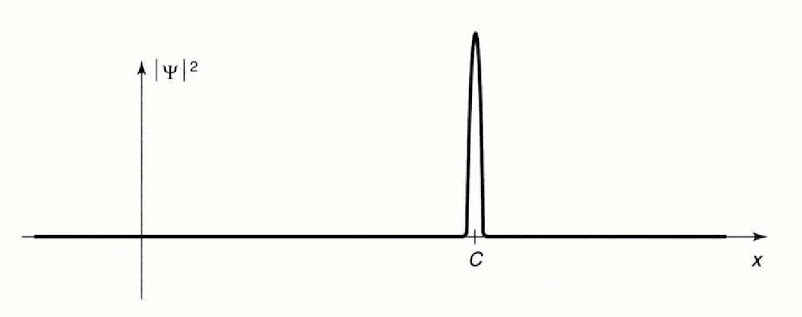
\includegraphics[scale=0.5]{griffiths_2.jpg}}
\caption{Illustration of the collapse of a wave function.}
\label{2}
\end{figure}
\section{Some Probability}
\begin{quote}
``So Einstein was wrong when he said, `God does not play dice.' Consideration of black holes suggests, not only that God does play dice, but that he sometimes confuses us by throwing them where they can't be seen.'' -- Stephen Hawking
\end{quote}
Because of the statistical interpretation of the wave function, we will need to have a few tools of probability at our disposal. Probability of discrete variables is fairly commonly known, but we will brush up on the basics here for completeness.
\subsection{Discrete Variables}
If, say, for $N$ people, $N(j)$ represents the number of people with age $j$. If we were to ask one of the $N$ people at random what their age was, the probability that they would have age $j$ is given by:
\begin{equation}
P(j) =  \frac{N(j)}{N}.
\end{equation}
We must have:
\begin{equation}
\sum_{j=0}^{\infty} P(j) = 1.
\end{equation}
The average value of $j$ (which we will write as: $\left<j\right>$) is given by:
\begin{equation}
\left< j \right> = \frac{\sum jN(j)}{N} = \sum_{j=0}^{\infty} j P(j).
\end{equation}
Now in quantum mechanics, the average is usually called the \emph{expectation value}. This is terrifically misleading terminology as it implies that this is is the outcome you would most likely get if you made a single measurement (the most probable measurement, not the average). Unfortunately physicists have already entrenched this bad habit, and we are stuck with it with calling it the expectation value.

In general, the average value of some function $f(J)$ is given by:
\begin{equation}
\left< f(j) \right> = \sum_{j=0}^{\infty}f(j)P(j).
\end{equation}
So, for example:
\begin{equation}
\left< j^{2} \right> = \sum_{j=0}^{\infty} j^{2}P(j).
\end{equation}
It is important to stress that $\left< j^{2} \right>$ and $\left< j \right>^{2}$ are not the same thing!

The standard deviation is a measure of how ``spread out'' a distribution is. Two distributions may have the same mean but one is spread out broad and flat around the mean while the other is sharply peaked at it. In this case, the former distributions will have a greater ``spread'' or standard deviation. We calculate the standard deviation from:
\begin{equation}
\sigma = \sqrt{\left< j^{2} \right> - \left< j \right>^{2}}.
\end{equation}
\subsection{Continuous Variables}
Probability of continuous variables is a bit less intuitive (at least to me) than probability of discrete variables. Instead of talking about the probability of a person's age being $j$, we now talk about how likely it is that their age is within some interval. If the interval is sufficiently short (this is eventually heading towards infinitesimal), the probability is \emph{proportional to the length of the interval}. For example: the chance that someone age is between 16 and 16 plus \emph{two} days is presumably twice the probability that it is between 16 and 16 plus \emph{one} day.\footnote{Unless their was a baby boom 16 years ago, in which case the interval is two long for the rule of thumb to apply.} So we have technically:
\begin{equation}
\rho (x) dx = \text{probability that an individual (chosen at random) lies between $x$ and $(x+dx)$}.
\label{probability_density_equation}
\end{equation}
Now, $\rho (x)$ is a proportionality factor, called the probability density. The probability that $x$ lies between $a$ and $b$ if given by the integral of $\rho (x)$:
\begin{equation}
P_{ab} = \int_{a}^{b} \rho (x) dx.
\end{equation}
The rules for discrete distributions generalise as follows:
\begin{eqnarray}
\label{unity}
1 &=& \int_{-\infty}^{+\infty}\rho (x) dx, \\
\label{expectation_value}
\left< x \right> &=& \int_{-\infty}^{+\infty} x \rho (x) dx, \\
\left< f(x) \right> &=& \int_{-\infty}^{+\infty} f(x)\rho (x) dx, \\
\sigma^{2} & \equiv & \left< \left( \Delta x\right)^{2}\right> = \left< x^{2} \right> - \left< x \right>^{2}.
\end{eqnarray}

\noindent\makebox[\linewidth]{\rule{\textwidth}{0.4pt}}
\textbf{Example 1:} Suppose we drop a rock off a cliff of height $h$. As it falls, we snap a million photographs at random intervals. On each picture I measure the distances the rock has fallen. \emph{Question}: What is the \emph{average} of all these distances? That is to say, what is the \emph{time average} of the distance traveled?

\textbf{Solution:}
The rock will start out at rest and gain speed as it falls. We will ignore air resistance. The distance $y$ at time $t$ is given by:
\begin{equation}
y(t) = \frac{1}{2}gt^{2}.
\end{equation}
The velocity is the derivative of the distance, $dy/dt$, and the total flight time is $T = \sqrt{2h/g}$. Now the probability that the camera flashes in the interval $dt$ is $dt/T$. Using all of this. the probability that a given photograph shows a distance in the corresponding range $dx$ is given by:
\begin{equation}
\frac{dt}{T} = \frac{dx}{gt}\sqrt{\frac{g}{2h}} = \frac{1}{2\sqrt{hx}}dx.
\end{equation}
We can then see from equation \ref{probability_density_equation} that the probability density is:
\begin{eqnarray}
\rho (x) = \frac{1}{2\sqrt{hx}}, & (0 \geq x \geq h)
\end{eqnarray}
(outside the range the probability density is zero). We can check this result using equation \ref{unity}:
\begin{equation}
\int_{0}^{h} \frac{1}{2\sqrt{hx}}dx = \frac{1}{2\sqrt{h}} \left( 2x^{1/2} \right) \Big|^{h}_{0} = 1.
\end{equation}
We can now get the \emph{average} distance using equation \ref{expectation_value}:
\begin{equation}
\left< x \right> = \int_{0}^{h} x \frac{1}{2\sqrt{hx}}dx = \frac{1}{2\sqrt{h}}\left( \frac{2}{3} x^{3/2} \right) \Big|^{h}_{0} = \frac{h}{3}.
\end{equation}
Figure \ref{3} shows the graph of $\rho (y)$. Note that the probability density itself can be infinite, though the probability (the integral of the probability density) itself must be $ \leq 1$.
\begin{figure}[h]
\centering{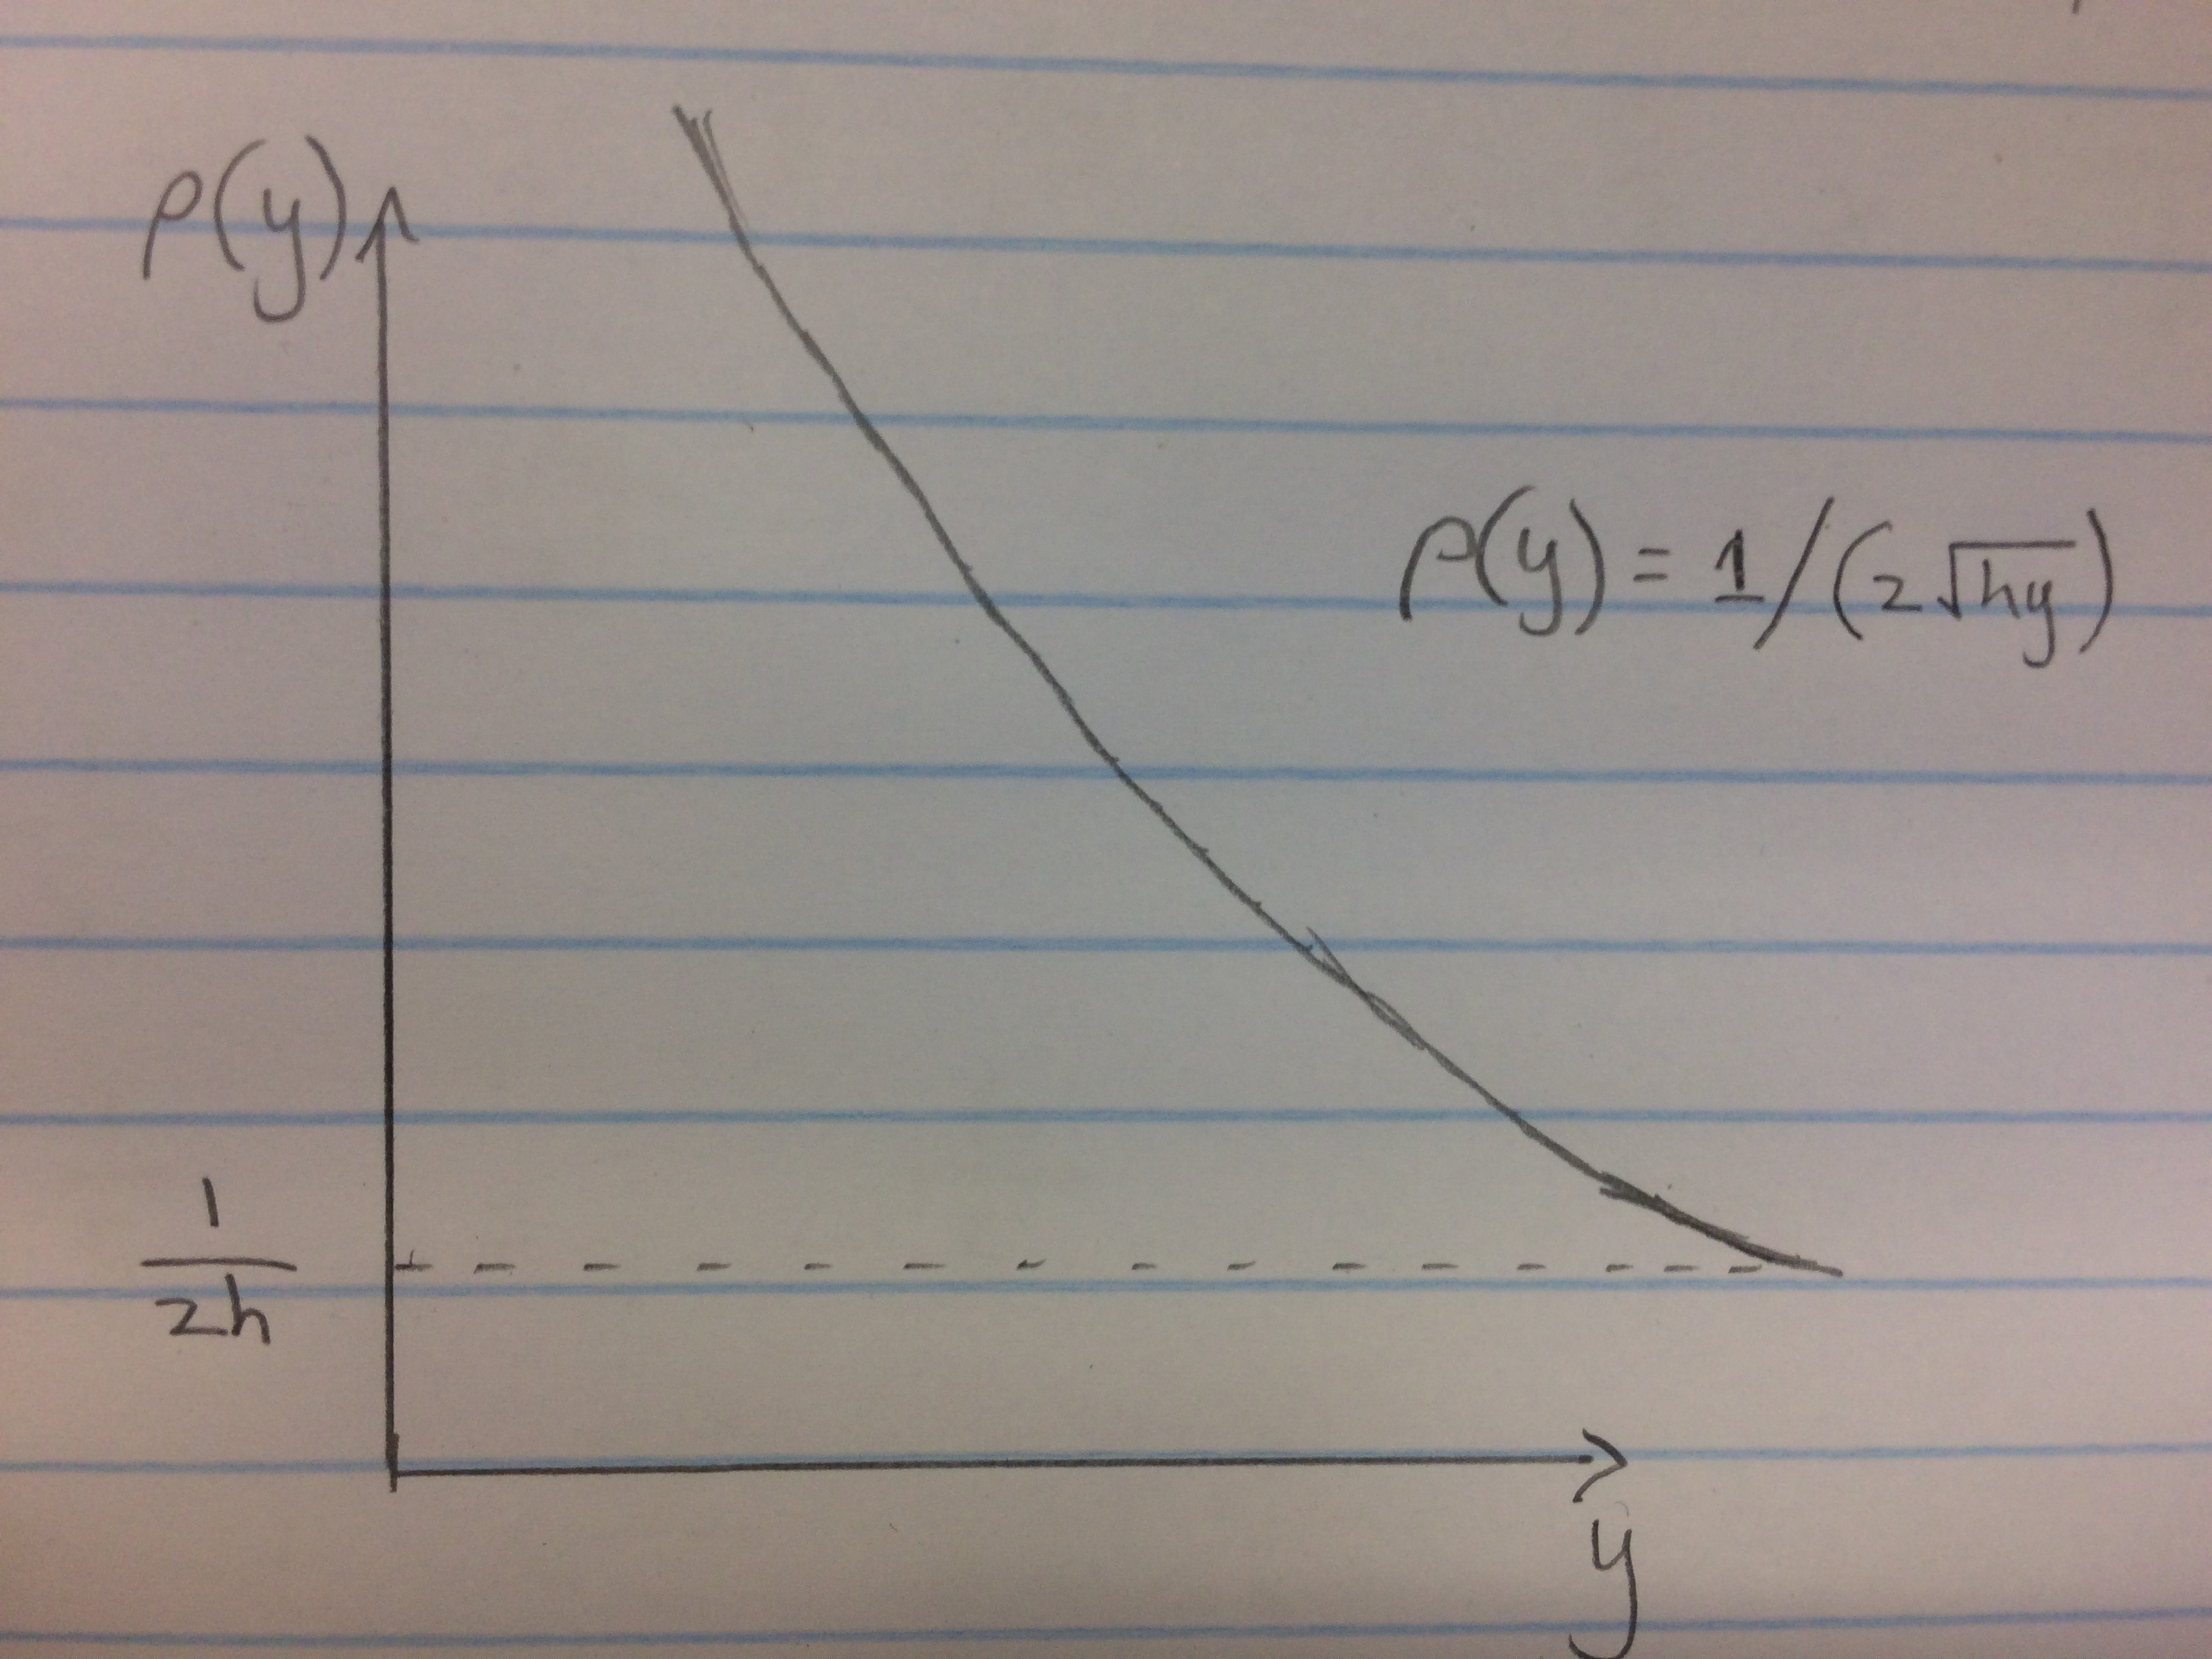
\includegraphics[scale=0.075]{griffiths_3.jpg}}
\caption{The probability density in Example 1.}
\label{3}
\end{figure}
\section{Normalisation}
\begin{quote}
[I can't accept quantum mechanics because] ``I like to think the moon is there even if I am not looking at it.'' -- Albert Einstein
\end{quote}
We now return to the statistical interpretation of the wave function, equation \ref{statistical_interpretation}. If $|\Psi (x,t)|^{2}$ is the probability density for finding the particle at point $x$, at time $t$; then we should have:
\begin{equation}
\label{normalised}
\boxed{\int_{-\infty}^{+\infty} \left| \Psi (x,t) \right|^{2}dx = 1.}
\end{equation}
If this wasn't true, then the statistical interpretation would be nonsense!

However, this is actually a bit troubling. If we get $\Psi$ from solving the Schrodinger equation, then we should check that this extraneous condition is consistent with it. If we examine equation \ref{schrodinger_equation} (the Schrodinger equation), we can see that if has the property that if $\Psi(x,t)$ is a solution, then so too is $A \Psi(x,t)$, where $A$ is any complex constant. What we must do then is pick this undetermined multiplicative factor so as to ensure that equation \ref{normalised} is satisfied. This process is called \textbf{normalising} the wave function. For some solutions to the Schrodinger equation, the integral is \emph{infinite} and as such no multiplicative factor is going to make it 1. The same goes for the trivial solution $\Psi = 0$. Such \textbf{non-normalisable} solutions cannot represent particles and must be rejected. Physically realisable solutions correspond to the \textbf{square-integrable} solutions to the Schrodinger equation. Hang on though. If we normalise the wave function at time $t=0$, then how do we know it will stay normalised as time goes on and $\Psi$ evolves? Because if we keep renormalising the wave function, the $A$ becomes a function of $t$, and we no longer have a solution to the Schrodinger equation. We are very fortunate in that the Schrodinger equation automatically preserves the normalisation of the wave function. Otherwise, quantum mechanics would break(down).

This is something worth proving, so here we go. Let's begin with:
\begin{equation}
\label{normalisation_proof}
\frac{d}{dt}\int_{-\infty}^{+\infty} \left| \Psi (x,t) \right|^{2}dx =\int_{-\infty}^{+\infty} \frac{\partial}{\partial t}\left| \Psi (x,t) \right|^{2}dx.
\end{equation}
Note that the \emph{integral} is a function only of $t$ and hence we use a \emph{total} derivative $(d/dt)$, but the \emph{integrand} is a function of $x$ as well as $t$ and hence the \emph{partial} derivative $(\partial/\partial t)$. From the product rule, we have:
\begin{equation}
\frac{\partial}{\partial t} | \Psi |^{2} = \frac{\partial}{\partial t} \left( \Psi^{*}\Psi \right) = \Psi^{*}\frac{\partial \Psi}{\partial t} + \frac{\partial \Psi^{*}}{\partial t}\Psi.
\end{equation}
Now, the Schrodinger equation says that:
\begin{equation}
\frac{\partial \Psi}{\partial t} = \frac{i\hbar}{2m}\frac{\partial^{2}\Psi}{\partial x^{2}} - \frac{i}{\hbar}V\Psi,
\end{equation}
and hence also (if we take its complex conjugate):
\begin{equation}
\frac{\partial \Psi^{*}}{\partial t} = -\frac{i\hbar}{2m}\frac{\partial^{2}\Psi^{*}}{\partial x^{2}} + \frac{i}{\hbar}V\Psi^{*},
\end{equation}
so
\begin{equation}
\label{griffiths_125}
\frac{\partial}{\partial t}|\Psi |^{2} = \frac{i\hbar}{2m}\left( \Psi^{*}\frac{\partial^{2}\Psi}{\partial x^{2}} - \frac{\partial^{2}\Psi^{*}}{\partial x^{2}}\Psi \right) = \frac{\partial}{\partial x} \left[ \frac{i\hbar}{2m}\left( \Psi^{*}\frac{\partial \Psi}{\partial x} - \frac{\partial \Psi^{*}}{\partial x}\Psi \right) \right].
\end{equation}
The integral in equation \ref{normalisation_proof} can now be evaluated explicitly:
\begin{equation}
\frac{d}{dt}\int_{-\infty}^{+\infty}| \Psi (x,t) |^{2}dx = \frac{i\hbar}{2m}\left( \Psi^{*}\frac{\partial \Psi}{\partial x} - \frac{\partial \Psi^{*}}{\partial x}\Psi \right)\Big|_{-\infty}^{+\infty}.
\end{equation}
But $\Psi (x,t)$ must go to zero as $x$ goes to $(\pm)$ infinity -- otherwise the wave function would not be normalisable\footnote{It seems that you also need to assume that the first derivate goes to zero at $\pm \infty$ too. Griffiths doesn't explicitly mention this here and I don't remember it. Why? Must look into it later. For now, take it as another axiom. It makes sense, I guess, provided that the wave function decays out to the tails. Then it makes sense that the slope would also go to zero. This just seems so mathematically inelegant.}. It follows that:
\begin{equation}
\frac{d}{dt} \int_{-\infty}^{+\infty} | \Psi (x,t)|^{2} dx = 0,
\end{equation}
and hence that the integral is \emph{constant} (independent of time); if $\Psi$ is normalised at $t=0$, it stays normalised for all future times.

\noindent\makebox[\linewidth]{\rule{\textwidth}{0.4pt}}
\textbf{Problem 1:} At time $t=0$ a particle is represented by the wave function:
\begin{equation}
\Psi(x,0) = \begin{cases}
A \frac{a}{a} & \text{if, } 0 \leq x \leq a, \\
A \frac{(b-x)}{(b-a)}, & \text{if, } a \leq x \leq b,  \\
0, & \text{otherwise},
\end{cases}
\end{equation}
where $A$, $a$, and $b$ are constants.
\begin{enumerate}[label=(\alph*), labelindent=\parindent,leftmargin=*]
\item Normalise $\Psi$ (i.e. find $A$ in terms of $a$ and $b$).
\item Sketch $\Psi(x,0)$ as a function of $x$.
\item Where is the particle most likely to be found at $t=0$.
\item What is the probability of finding the particle to the left of $a$? Check the result in the limiting cases $b=a$ and $b=2a$.
\item What is the expectation value of $x$?
\end{enumerate}
\noindent\makebox[\linewidth]{\rule{\textwidth}{0.4pt}}
\textbf{Problem 2:} Consider the wave function:
\begin{equation}
\Psi(x,t) = Ae^{-\lambda|x|}e^{-i\omega t},
\end{equation}
where $A$, $\lambda$, and $\omega$ are positive real constants.
\begin{enumerate}[label=(\alph*), labelindent=\parindent,leftmargin=*]
\item Normalise $\Psi$.
\item Determine the expectation values of $x$ and $x^{2}$.
\item Find the standard deviation of $x$. Sketch the graph of $| \Psi |^{2}$, as a function of $x$, and mark the points $(\left< x \right> + \sigma)$ and $(\left< x \right> - \sigma)$, to illustrate the sense in which $\sigma$ represents the ``spread'' in $x$. What is the probability that the particle would be found outside this range?
\end{enumerate}
\section{Momentum}
\begin{quote}
``Quantum theory provides us with a striking illustration of the fact that we can fully understand a connection though we can only speak of it in images and parables.'' -- Werner Heisenberg
\end{quote}
Recall that the expectation value of a particle in state $\Psi$ is given by:
\begin{equation}
\left< x \right> = \int_{-\infty}^{+\infty} x | \Psi (x,t) |^{2} dx.
\end{equation}
We should pause for a moment to consider what this means. You may think that it means that if we measured the position of the particle over and over again, this is the average of the measurements we would get. This is NOT however correct. $\left< x \right>$ is the average of measurements performed on particle \emph{who are all in state $\Psi$}. You can think of it as the average value of measurements performed on an \textbf{ensemble} of particles all in state $\Psi$. Think of 100 bottles (or universes), each containing a particle in state $\Psi$. We politely ask a group of hard-working post-grads to take a ruler and measure the position of the particles simultaneously in all the bottles. The average of all of these measurements is what we are referring to.

Now, as time goes on, $\left< x \right>$ will change (it will evolve in time according to the Schrodinger equation), it might be interesting to know how fast it changes. Employing equation \ref{griffiths_125}, we see that\footnote{Let's suppress the limits of integration to make things look less messy.}:
\begin{equation}
\frac{d\left< x \right>}{dt} = \int x \frac{\partial}{\partial t} | \Psi |^{2} dx = \frac{i\hbar}{2m}\int x \frac{\partial}{\partial x} \left( \Psi^{*}\frac{\partial\Psi}{\partial x} - \frac{\partial \Psi^{*}}{\partial x}\Psi \right) dx.
\end{equation}
We can simplify using integration by parts:
\begin{equation}
\frac{d \left< x \right>}{dt} = -\frac{i\hbar}{2m}\int \left( \Psi^{*}\frac{\partial \Psi}{\partial x} - \frac{\partial \Psi^{*}}{\partial x} \Psi \right) dx,
\end{equation}
(using the fact that $\partial x / \partial x = 1$, and that the boundary terms go to zero at $\pm \infty$). If we use integration by parts again, on the second term, then we have:
\begin{equation}
\frac{d\left< x \right>}{dt} = -\frac{i\hbar}{m}\int\Psi^{*}\frac{\partial \Psi}{\partial x}dx.
\end{equation}
This is the velocity of the expectation value of $x$, not to be confused with the actual velocity of the particle. It is possible to construct the probability density for the particle's velocity, though it is outside the scope of these notes. Suffice then to postulate that the \emph{expectation value of the velocity is equal to the time derivative of the expectation value of position}:
\begin{equation}
\left< x \right> = \frac{d\left< x \right>}{dt}.
\end{equation}
This equation tells us how to calculate $\left < v \right>$ directly from $\Psi$. Physicists generally prefer to work with momentum ($p=mv$) instead of velocity:
\begin{equation}
\label{momentum}
\left< p \right> = m\frac{d\left< x \right>}{dt} = -i\hbar \int \left( \Psi^{*}\frac{\partial \Psi}{\partial x} \right) dx.
\end{equation}

A quantity related to a particle is called an observable. In quantum mechanics, all observable are represented by \emph{linear operators}\footnote{Linear operators as defined in linear algebra.}. We can find the expectation value of any observable by sandwiching the operator that corresponds to that observable between $\Psi^{*}$ and $\Psi$ and integrating. The operator for position is just $x$ and, looking at equation \ref{momentum} for inspiration, the momentum operator is $-i\hbar$ $\partial/\partial x$. So the expectation variables for these observables are given by:
\begin{eqnarray}
\left< x \right> &=& \int \Psi^{*} (x) \Psi dx, \\
\left< p \right > &=& \int \Psi^{*} \left( \frac{\hbar}{i} \frac{\partial}{\partial x} \right) \Psi dx.
\end{eqnarray}
All classical dynamical variables can be expressed in terms of position and momentum. Kinetic energy, for example, is given by:
\begin{equation}
T = \frac{1}{2}mv^{2} = \frac{p^{2}}{2m}.
\end{equation}
Then the expectation value of the kinetic energy is given by:
\begin{equation}
\left< T \right > = - \frac{\hbar^{2}}{2m} \int \Psi^{*}\frac{\partial^{2}\Psi}{\partial x^{2}} dx.
\end{equation}
In general, the expectation value for any quantity $Q(x,p)$ can be found using:
\begin{equation}
\boxed{\left< Q(x,p) \right> = \int \Psi^{*} Q \left( x,\frac{\hbar}{i}\frac{\partial}{\partial x} \right) \Psi dx.}
\end{equation}

\noindent\makebox[\linewidth]{\rule{\textwidth}{0.4pt}}
\textbf{Problem 3:} Calculate $d\left< p \right> / dt$. \emph{Answer:}
\begin{equation}
\frac{d\left< p \right>}{dt} = \left< - \frac{\partial V}{\partial x} \right>.
\end{equation}
This is an example of \emph{Ehrenfest's theorem} which says that \emph{expectation values obey classical laws}.
\section{The Uncertainty Principle}
\begin{quote}
``We demand rigidly defined areas of doubt and uncertainty!'' -- Douglas Adams, The Hitchhikers Guides to the Galaxy
\end{quote}
And now, we reach the famous Heisenberg uncertainty principle. It's derivation is fairly complicated and relies on a lot of concepts and ideas from linear algebra, so we will not derive it here. Instead, we will focus on understanding what it means. The analogy Griffiths uses is one of a rope. Say we take a long rope (say 50 metres) and you hold one end and I hold the other. I begin the rhythmically shake the rope up and down and this results is a series of wave traveling down the length of the rope. If I asked you `Where is the wave?', you would no doubt think this is a bit of a silly question. The wave isn't really anywhere, it's spread out across the whole length of the rope. But if I asked you what the wavelength of the wave is, then you could certainly give me a reasonable answer. `It looks like 6 metres.' say. On the other hand, if I take the rope and give it a sudden jerk, it will results in a single narrow bump traveling down the length of the rope. Now the question of where the wave is seems reasonable, where the question of what the wavelength is seems silly. There's a trade-off. If the wavelength is well defined, then the position is inversely ill-defined and vice versa. This can all be made rigorous by using Fourier analysis but that is outside the scope of why we're here. This is, however, a nice qualitative argument that applies to any wave phenomena, including the quantum mechanical wave function.

Now, the wave function of $\Psi$ is related to the \emph{momentum} of the particle by the \textbf{de Broglie formula}:
\begin{equation}
p = \frac{h}{\lambda} = \frac{2\pi\hbar}{\lambda}
\end{equation}
Hence, a spread in \emph{wavelength}, corresponds to a spread in \emph{momentum}. So the more precisely defined a particle's position is, the less precisely its momentum is. Quantitatively:
\begin{equation}
\boxed{\sigma_{x}\sigma_{p} \geq \frac{\hbar}{2}},
\end{equation}
where $\sigma_{x}$ is the standard deviation in $x$, and $\sigma_{p}$ is the standard deviation in $p$. 

This is the famous \textbf{Heisenberg's Uncertainty Principle}. Let's think about what it means: momentum, like position, yields precise answers for when it's measured. The ``spread'' here refers to the fact that measurements on identically prepared systems do not yield identical results. You can, if you want, construct a state such that repeated position measurements will be very close together (by making $\Psi$ a very localised spike), but you will pay a price: Momentum measurements on this state will be wide scattered. Conversely, you can prepare a state with a reproducible momentum (by making $\Psi$ a long sinusoidal wave), but then position measurements will be widely scattered. And, of course, since it's an inequality, would could just make it a big mess with very scattered measurements for both position and momentum.

\noindent\makebox[\linewidth]{\rule{\textwidth}{0.4pt}}
\textbf{Problem 4:} A particle of mass $m$ is in state:
$$ \Psi(x,t) = Ae^{-a[(mx^{2}/\hbar)+it]},$$
where $A$ and $a$ are positive real constants.
\begin{enumerate}[label=(\alph*), labelindent=\parindent,leftmargin=*]
\item Find $A$.
\item For what potential energy function $V(x)$ does $\Psi$ satidy the Schrodinger equation?
\item Calculate the expectation values of $x,$, $x^{2}$, $p$, and $p^{2}$.
\item Find $\sigma_{x}$ and $\sigma_{p}$. Is their product consistent with the uncertainty principle?
\end{enumerate}
\newpage
\section{The Standard Model of Particle Physics}
The Standard Model (see figure \ref{sm_part_image}) of particle physics was developed in the latter half of the twentieth century. It describes how matter is comprised of point-like, basic building blocks, called fundamental particles, which interact via three fundamental forces. The Standard Model has been tested successfully many times and is widely regarded as the most accurate and stable model of particle physics. It classifies the fundamental particles that make up matter into either leptons or quarks. Both leptons and quarks come in three so-called generations, with the members of the later generations being heavier and less stable than their previous generation counterparts.\footnote{An important caveat to this are the neutrinos, which do not decay, and whose tiny non-zero mass is not known to be related to their generation.}. In ascending order of generation, the leptons are: the electron and electron neutrino, the muon and muon neutrino, and the tau and tau neutrino. Quarks are also classified into three generations, with each generation having two flavours of quarks. In ascending order of generation, the quarks are: the up and down, the charm and strange, and the top and bottom. Quarks are never observed in isolation due to colour confinement and instead are only observable in bound states called hadrons. Bound states consisting of a quark-antiquark pair are called mesons, while bound states of three quarks are called baryons. Both leptons and quarks have half-integer spin. Particles possessing half-integer spin are known collectively as \emph{fermions}. Fermions as a collective are constrained by the Pauli exclusion principle, meaning that no two fermions may occupy the same quantum state.

The Standard Model describes three of the four fundamental interactions in nature. In increasing order of strength, these are: the weak, electromagnetic, and strong forces. According to the Standard Model: the strong, weak, and electromagnetic forces result from the exchange of force-carrier particles. These force carriers possess integer-spins  and are collectively called \emph{bosons}. Specific bosons are said to mediate a particular force. The strong force is mediated by the gluon, the electromagnetic by the photon, and the weak by the W and Z bosons. The masses of the elementary particles arise from their coupling to the Higgs field, which is mediated by the Higgs boson.

The process via which fundamental particles couple to the Higgs field and hence become massive is called the \emph{Higgs mechanism}. The Higgs boson was experimentally observed by the ATLAS and CMS collaborations in 2012. At extremely hot temperatures\footnote{When the equilibrium thermal energy of the system is on the order of 100 GeV.} the W and Z bosons are effectively massless and the electromagnetic and weak forces become practically indistinguishable. They are, in fact, different aspects of the same unified electroweak force or \emph{electroweak interaction}. Below the aforementioned sufficiently high temperature, this symmetry is spontaneously broken, resulting in the W and Z bosons having mass via the Higgs mechanism and making the electromagnetic and weak forces appear distinct. Both the strong and electroweak interactions are described by their corresponding \emph{gauge theories}, with \emph{Quantum ChromoDynamics} (QCD) describing the former and \emph{electroweak field theory} describing the latter.

A deficiency of the Standard Model is that it does not describe the gravitational interaction. Theories that seek to expand upon the Standard Model in order to, for example, incorporate gravity are said to be ``beyond'' the Standard Model.
\begin{figure}[h]
\centering
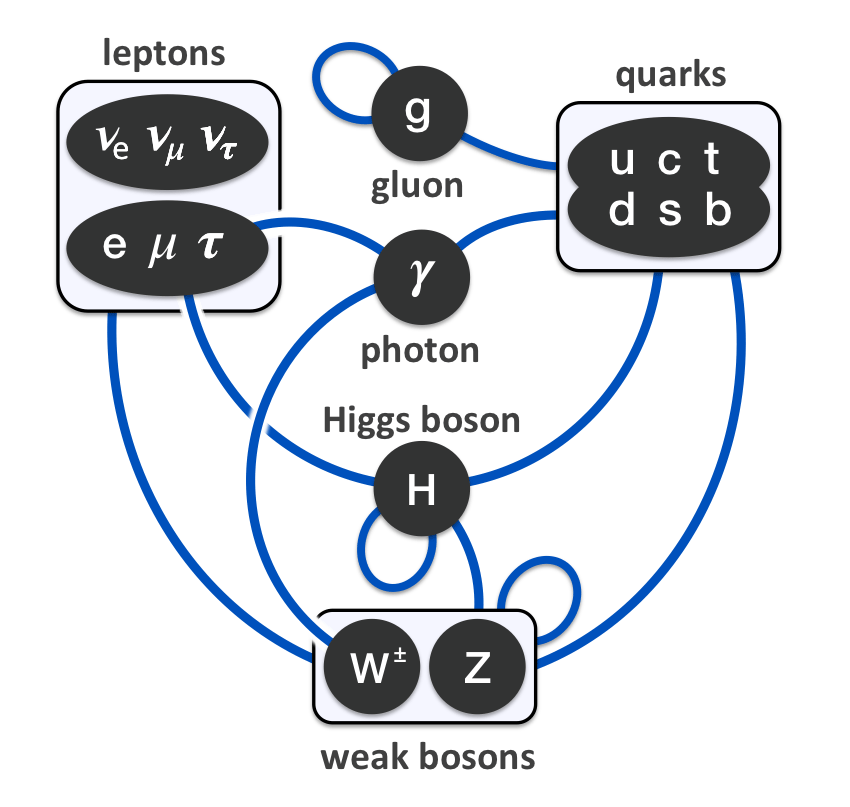
\includegraphics[width=0.55\textwidth]{../thesis/images/fund_part_in_sm.png}
\label{sm_part_image}
\caption{Illustration of the fundamental particles described by the Standard Model, showing how they interact amongst each other and sometimes themselves.}
\end{figure}
\newpage
\section{The Many Worlds Interpretation of Quantum Mechanics}
We will begin by going over the general concept of coherence, before moving onto quantum decoherence, and then finally we will discuss the many worlds interpretation.

\begin{figure}[h]
\centering
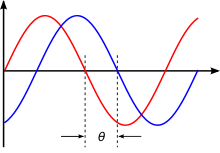
\includegraphics[width=0.35\textwidth]{phase_shift.png}
\caption{Illustration showing the phase shift $\theta$ between two sinusoidal waves.}
\label{phase_shift}
\end{figure}

We must first quickly introduce wave phases. The phase of a sinusoidal wave is the initial value of the sinusoidal function at time $t=0$. For a sine graph of the general form $y(t) = A \sin \left( 2\pi f t + \phi \right)$, where $A$ is the sinusoidal wave's amplitude, $f$ is its frequency, and $\phi$ is its phase. Now, when we look at two  waves, of the same shape and frequency, on the same set of axes, the distance on the x-axis between the same point on each wave is called the \emph{phase shift} (see figure \ref{phase_shift}). If the phase shift is constant then the waves are said to be \emph{coherent}. This is important in the context of Young's famous double-slit experiment, where coherent waves of light (from a laser, say) pass through the double-slit producing light patterns on the incident screen. The light waves here interfere with each and result in a series of bright dots on the incident screen, corresponding to points where the waves constructively interfere with each other. Exactly how and where the waves will interfere with each other is dependent on the phase-shift between the coherent waves.

\begin{figure}[h]
\centering
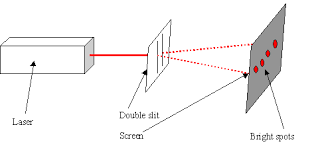
\includegraphics[width=0.55\textwidth]{youngs.png}
\caption{Illustration the classic Young's double-slit experiment, showing the constructive interference of coherent light-waves resulting in bright spots on the screen.}
\label{youngs}
\end{figure}

In quantum mechanics, all objects have wave-like properties (de Broglie waves). Hence, we can (and this has been done many times) use electrons in place of light for the double-slit experiment (see figure \ref{electron_youngs}). We shoot electrons using an electron gun at the slits and the electron-waves will constructively interfere to produce the same interference pattern as the light-waves! It actually gets even weirder at this point because if we place detectors at each of the slits to see what a passes though them, we see that the electrons just regularly pass through either one slit or the other and there is no interference pattern, only two ``clumps'' of electrons found on the screen directly across from each slit. So if we look to see what the electrons are doing at the slits, they behave as we would expect classically, like particles. But if we don't check up on them as they pass through the slit, then they behave like waves and create a wave interference pattern as we could expect quantumly.

Some physicists have tried to explain this strange phenomenon in terms of \emph{quantum decoherence}. Decoherence maintains that the act of bring a quantum system into contact with something macroscopic results in the quantum system leaking its ``quantumness'' into the macroscopic system. This is often modeled as an object being in contact with a heat bath. Decoherence poses challenges for quantum computing as they are going to rely on the fact that their quantum systems undisturbedly coherent. Now, it is really important to point out here that quantum decoherence does not solve the measurement problem in quantum mechanics, i.e. it doesn't attempt to generate wave function collapse. Rather it provides an explanation for the appearance of wave function collapse. Advocates of quantum decoherence will often refer to the so-called ``universal-wavefunction'' of which the whole universe in always in total superposition. They say that when we place the detectors at the slits, they essentially cause the quantum behaviour of the electrons to become lost and as a result that behave classically. Quantum decoherence by itself does not constitute an interpretation of quantum mechanics, but it forms an important part of some modern reformulations of the Copenhagen interpretation, as well as the many-worlds interpretation. Speaking of which...

\begin{figure}[h]
\centering
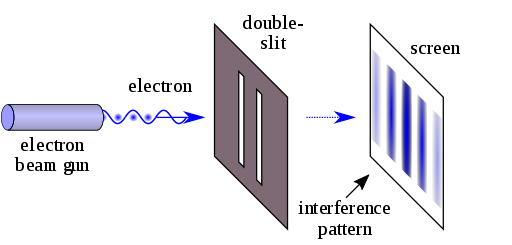
\includegraphics[width=0.55\textwidth]{electron_youngs.png}
\caption{Illustration the modern double-slit experiment, showing the constructive interference of coherent electron-waves resulting in spots indicated of constructive interference on the screen.}
\label{electron_youngs}
\end{figure}

This interpretation of quantum mechanics is often depicted in popular media and is frequently advocated in the interpretation debates. It was originally conceived of by an American PhD student Hugh Everett in 1957, but was popularised by Bryce DeWitt more than a decade later. It relies heavily on the concept of quantum decoherence. The many worlds interpretation (MWI) states the universal wavefunction is an objective reality and that all possible alternate histories and future are real, each constituting an actual separate universe. So in essence, anything that ever could have possibly happened in our past has happened in the past of another universe. It is a realist, deterministic, arguably local theory, which removes wavefunction collapse entirely and replaces it with quantum decoherence. Some other interpretations that involve quantum decoherence such as the consistent histories approach (a more modern version of the Copenhagen interpretation) or the existential approach, regard these ``parallel worlds'' are being metaphorical or are agnostic towards their physical existence. So if we think of Schrodinger's cat, in one universe we may find the cat alive, while in another far less cheerful one, we find it dead. The MWI is often presented as a theory rather than an interpretation by its strong advocates, particularly the Israeli-born Camebridge physicist David Deutch. He and his fellow many-worldians claim that it makes testable predictions, is falsifiable, and that other interpretations are inconsistent, illogical, or unscientific in their handling of measurements. With regards to MW as a theory rather than an interpretation, Deutch claims: ``[it's like] talking about dinosaurs as an interpretation of fossil records''. He claims that the interference patterns seen in the electron double slit experiment are evidence of the worlds interacting with each. Nevertheless, there is no consensus among physicists as to which interpretation of quantum mechanics is correct, and Deutch's sentiment on MW being a tested theory is certainly not agreed upon in the physics village. Those adhering to the Copenhagen interpretation claim that the interference pattern and quantum nature of the electrons is due to the fact that their wave function is not collapsed.
\end{document}